\section{Far Detector and Uncertainties}
%{\it Assigned to:} {\bf Dan Cherdack} with contributions from Nick Grant, Leigh Whitehead, Callum Wilkinson, Elizabeth Worcester and Tingjun Yang.
\label{sec:physics-lbnosc-FD}
%This section describes assumptions in the Near Detector simulation and reconstruction. Some thought has to go into the connection to the Far Detector chapter in the TDR.

%\begin{itemize}
%    \item Simulations - TY 
%    \item Reconstruction and kinematic variables including energy reconstruction - TY, NG 
%    \item Event selections (CVN) - LW
%    \item Samples - EW, CW
%    \item Detector response systematic uncertainties - DDC
%    \item Connection to flux and cross section systematic uncertainties
%\end{itemize}
\fixme{Needs intro text to Far Detector} 

\subsection{Simulation}
The neutrino samples were simulated using a smaller version of the full 10 kt far detector geometry. This geometry is 13.9 m long, 12 m high and 13.3 m wide, which consists of 12 APAs and 24 TPCs. The reference flux was used (Section~\ref{sec:physics-lbnosc-flux}) and samples were produced with both the forward-horn-current (neutrino enhanced) and inverted-horn-current (antineutrino enhanced) beam configurations. Three samples were generated. The first sample keeps the original neutrino flavor in the beam. The second sample converts all the muon neutrinos to electron neutrios. The third sample converts all the muon neutrinos to tau neutrinos. {\sc genie} \todo{name genie version} was used to model the neutrino-argon interactions in the volume of cryostat. The produced secondary particles were propagated in the detector through {\sc geant}. The ionization electrons and scintillation light were digitized to produce signals in the wire planes and photon detectors. More details on the simulation can be found in the Physics Tools and Methods chapter~\ref{}.

\subsection{Event reconstruction and kinematic variables}
The first step in the reconstruction is to convert the raw signal from each wire to a standard (e.g. Gaussian) shape. This is achieved by passing the raw data through a calibrated deconvolution algorithm to remove the impact of the LArTPC electric field and electronics responses from the measured signal.

The hit-finding algorithm scans the processed wire waveform looking for local minima. If a minimum is found, the algorithm follows the waveform after this point until it finds a local maximum. If the maximum is above a specified threshold, the program scans to the next local minimum and identifies this region as a hit. Hits are fit with a Gaussian function whose features identify the correct position (time coordinate), width and height and area (deposited charge) of the hit. A single Gaussian function is used to describe hits produced by isolated single particles. Multiple Gaussian functions are used to describe hits in a region where there are overlapping particles (e.g. around neutrino interaction vertex). The reconstructed hits are input to the CVN event selection described later.

Pattern recognition algorithms (Pandora and PMA) define clusters as hits that may be grouped together due to proximity to one another. Clusters from different planes are matched to form high-level objects such as tracks and showers, which are used as input to reconstruct the neutrino energy. More details on the reconstruction can be found in the Physics Tools and Methods chapter.

% Neutrino energy reconstruction

The energy of the incoming neutrino in charged-current events is estimated by adding the reconstructed lepton and hadronic energies. 
If the event is selected as $\nu_{\mu}$ CC, the 
neutrino energy is estimated as the sum of the energy of the longest reconstructed track and the hadronic energy. The energy of the longest reconstructed track is estimated from its 
range if the track is contained in the detector, and this is calibrated using simulated $\nu_{\mu}$ CC events. If the longest track exits the detector, its energy is estimated from 
multi-Coulomb scattering, and corrected using simulated events. The hadronic energy is estimated from the charges of reconstructed hits that 
are not in the longest track, and corrections are applied to each hit charge for recombination and the electron lifetime. An additional correction is then made to the hadronic energy to account for missing energy due to neutral particles and final-state interactions, and this is done using simulated events. 

If the event is selected as $\nu_{e}$ CC, the energy of the 
neutrino is estimated as the sum of the energy of the reconstructed shower with the highest energy and the hadronic energy. The former is estimated from the charges of the reconstructed 
hits in the shower, and the latter from the hits not in the shower; the recombination and electron lifetime corrections are applied to the charge of each hit. Subsequently the shower 
energy is corrected using simulated events, and the missing energy correction is applied to the hadronic energy.

The fractional residuals of reconstructed $\nu_{e}$ energy in $\nu_{e}$ CC events are shown in figure \ref{fig:enresnue}, and the biases and resolutions of reconstructed neutrino energy 
are summarised in table \ref{tab:ressummary}.

\begin{figure}[h]
    \centering
        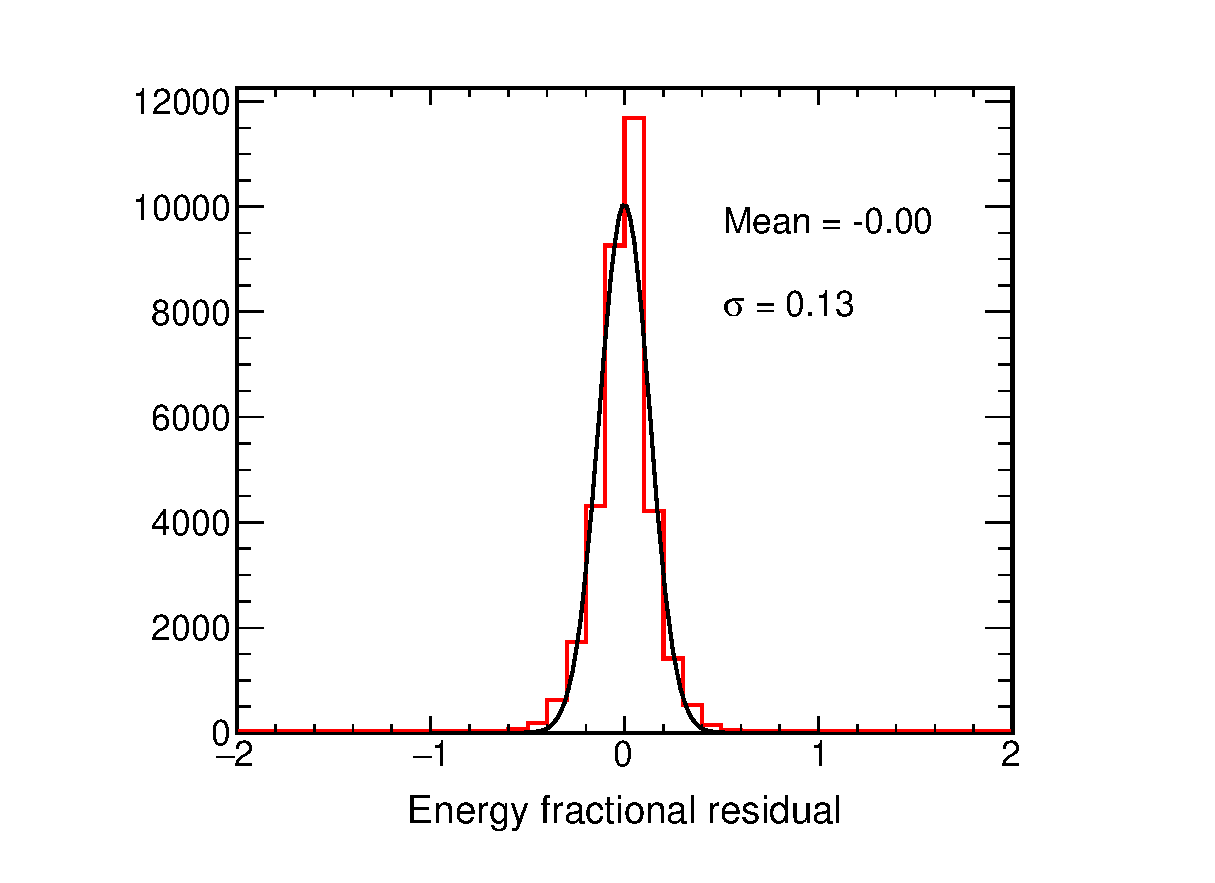
\includegraphics[width=0.55\textwidth]{EnergyResNue.eps}
        \caption{Fractional residuals of reconstructed $\nu_{e}$ energy in $\nu_{e}$ CC events}
        \label{fig:enresnue}
\end{figure}

\begin{table}[h]
\begin{center}
\begin{tabular}{|c|c|c|}
\hline  
 Event selection  &   Bias (\%) & Resolution (\%) \\ \hline
\hline
 $\nu_{\mu}$ CC with contained track  &   -1  &  18   \\ \hline
 $\nu_{\mu}$ CC with exiting track  &  -4   &  20 \\ \hline
 $\nu_{e}$ CC    &  0 & 13    \\ \hline
\end{tabular}
\caption{Summary of biases and resolutions of reconstructed neutrino energy}
\label{tab:ressummary}
\end{center}
\end{table}

% Start DUNE CVN event selection subsection from Leigh and Saul

\subsection{Neutrino event selection using the CVN}
The DUNE Convolutional Visual Network (CVN) classifies neutrino interactions in the DUNE FD through image recognition techniques. In general terms it is a convolutional neural network (CNN). Similar techniques have been demonstrated to outperform traditional methods in many aspects of high energy physics~\cite{radovicNature}.

The primary goal of the CVN is to efficiently and accurately produce event selections of the following interactions: CC$\nu_\mu$ and CC$\nu_e$ in the FHC beam mode, and CC$\bar{\nu}_\mu$ and CC$\bar{\nu}_e$ in the RHC beam mode. Future goals will include studies of exclusive neutrino interaction final states since separating the event selections by interaction type can improve the sensitivity as interaction types have different energy resolutions and systematic uncertainties.

Detailed descriptions of the CVN architecture can be found in Ref.~\cite{cvnPaper}.

\subsubsection{Network architecture}
The CVN design is based on the SE-ResNet architecture, which consists of a standard ResNet (Residual neural network) architecture~\cite{He-et-al-2015-deep} along with Squeeze-and-Excitation blocks~\cite{Hu-et-al-2017-squeeze}. Residual neural networks allow the $n^{th}$ layer access to the output of both the $(n-1)^{th}$ layer and the $(n-k)^{th}$ layer via a residual connection, where $k$ is a positive integer $>=2$. This is an important feature for the DUNE CVN as it allows the fine-grained detail of a LArTPC encoded in the input images to be propagated further into the CVN than would be possible using a traditional CNN such as the GoogLeNet (also called Inception v1)~\cite{GoogLeNet} inspired network used by NOvA~\cite{novacvn}.

\subsubsection{Inputs to the CVN}
\label{sec:inputs}
Three images of the neutrino interactions are produced where each image shows the event in one of the three readout views. These images are produced using the reconstructed hits on the individual wire planes and are not dependent on any further downstream reconstruction algorithms. The images contain 500$\times$500 pixels each in the (wire, time) parameter space where the wire is the wire channel number and the time is the peak time of the reconstructed hit measured in TDCs. The value of each pixel represents the integrated charge of the reconstructed hit. An example 2.2\,GeV CC$\nu_e$ interaction is shown in all three views in Fig.~\ref{fig:views} demonstrating the fine-grained detail available from the LArTPC technology.

\begin{figure}[htb] 
	\begin{tabular}{ccc}
		\includegraphics[scale=0.3]{cvn_nue_view0.pdf} &
		\includegraphics[scale=0.3]{cvn_nue_view1.pdf} &
		\includegraphics[scale=0.3]{cvn_nue_view2.pdf}
    \end{tabular}
	\caption{A 2.2\,GeV CC$\nu_e$ interaction shown in the three readout views of the DUNE LArTPCs. The horizontal axis shows the wire number of the readout plane and the vertical axis shows time. The colour scale shows the charge of the energy deposits on the wires.}
	\label{fig:views}
\end{figure}

\subsubsection{Training the CVN}
\label{sec:training}

The CVN was trained using approximately 3 million neutrino interactions from the Monte Carlo simulation that are independent of the sample that is used to generate the physics measurement sensitivities. The sample was chosen to ensure similar numbers of training examples from the different neutrino flavours. The CVN was trained ensuring that similar classification performance was obtained for the training and test samples (i.e ensure that the CVN was not overtrained).

\subsubsection{Outputs from the CVN}
\label{sec:outputs}

The CVN has six different outputs:
\begin{itemize}
    \item Primary output - neutrino flavour: returns probabilities that each interaction is one of the following classes: CC$\nu_\mu$, CC$\nu_e$, CC$\nu_\tau$ and NC.
    \item Four particle counting outputs for protons, charged pions, neutral pions and neutrons. Probabilities are returned for the presence of 0, 1, 2 and $>2$ particles of each aforementioned type.  
    \item Neutrino / antineutrino discriminator: returns the probability for the interaction to be an antineutrino.
\end{itemize}

As stated, all of the outputs are probabilities that allow neutrino event selections to be easily defined.

\subsubsection{Neutrino flavour identification}
The primary goal of the CVN is to accurately identify CC$\nu_e$ interactions and CC$\nu_\mu$ interactions to allow for the selection of the samples required for the neutrino oscillation analysis. The CC$\nu_e$ probability distribution, $P(\textrm{CC}\nu_e)$, and the CC$\nu_\mu$ probability distribution, $P(\textrm{CC}\nu_\mu)$, are shown on the left and right of Fig.~\ref{fig:cvnprob}, respectively. Excellent separation between the signal and background interactions is seen in both cases.

\begin{figure}
    \centering
    \begin{tabular}{cc}
%		\includegraphics[width=0.45\linewidth]{cvn_nue_prob_log.pdf} &
%		\includegraphics[width=0.45\linewidth]{cvn_numu_prob_log.pdf} 
	\end{tabular}
%	\caption{The neutrino flavour classification probabilities $P(\nu_e)$ (left) and $P(\nu_\mu)$ (right) for FHC-mode simulated CC$\nu_\mu$ (purple), CC$\nu_e$ (green), CC$\nu_\tau$ (cyan) and NC (orange) neutrino interactions.}
	\caption{The CVN CC$\nu_e$ probability (left) and CC$\nu_\mu$ probability (right) for the FHC beam mode shown with a log scale.}
    \label{fig:cvnprob}
\end{figure}
\fixme{Anne commented out figures because they're absent. 1/9}

The CC$\nu_e$ event selection requires $P(\textrm{CC}\nu_e) > 0.85$ for an interaction to be considered a CC$\nu_e$ candidate event. Similarly, interactions are selected as CC$\nu_\mu$ candidates if $P(\textrm{CC}\nu_\mu) > 0.5$. Note that since all of the flavour classification probabilities must sum to one, the interactions selected in the two event selections are completely independent. The same selection criteria are used for both FHC and RHC beam modes. The values used in the selection criteria were optimised to produce the best $\delta_{CP}$ sensitivity.

Figure~\ref{fig:nueeff} shows the efficiency as a function of reconstructed energy (under the electron neutrino hypothesis) for the $\nu_e$ event selection. The efficiency in both the FHC and RHC beam modes exceeds 90\% in the neutrino flux peak, with a clear improvement in the main region of interest over the efficiency presented in the DUNE CDR. Figure~\ref{fig:numueff} shows the corresponding excellent selection efficiency for the $\nu_\mu$ event selection.

\begin{figure}
    \centering
%    \begin{tabular}{cc}
		\includegraphics[scale=0.4]{cpv_compare_effs_cvnvcdr_dec2018.png} %&
		%\includegraphics[scale=0.22]{cvn_placeholder.pdf} 
%	\end{tabular}
	\caption{The CC$\nu_e$ selection efficiency for FHC-mode (top) and RHC-mode (bottom) simulation with the criterion $P(\textrm{CC}\nu_e) > 0.85$. The solid (dashed) lines show results from the CVN (CDR) for signal CC$\nu_e$ and CC$\bar{\nu}_e$ events in black and NC background interaction in red. The yellow region shows the oscillated flux to illustrate the most important regions of the energy distribution.}
    \label{fig:nueeff}
\end{figure}

\begin{figure}
    \centering
    \begin{tabular}{cc}
		\includegraphics[width=0.45\linewidth]{numu_eff_fhc.eps} &
		\includegraphics[width=0.45\linewidth]{numu_eff_rhc.eps} 
	\end{tabular}
	\caption{The CC$\nu_\mu$ selection efficiency for FHC-mode (left) and RHC-mode (right) simulation with the requirement $P(\textrm{CC}\nu_\mu) > 0.5$. (Describe the various colours).}
    \label{fig:numueff}
\end{figure}

\subsubsection{Exclusive final states}
The CVN has four outputs that count the number of final-state particles for the following species: protons, charged pions, neutral pions and neutrons. Neutrino interactions with different final-state particles can have varying energy resolutions depending on the complexity and particle multiplicity of the interaction. The ability to accurately select exclusive final-states will allow for those interactions with very good energy resolution to be fully exploited in the oscillation fit to improve the sensitivity of the analysis.

The individual output probabilities from the CVN can be multiplied together to give probabilities for exclusive selections. For example, Fig.~\ref{fig:exclusive} shows the CC$\nu_\mu$ 1 proton probability on the left formed by the product 
\begin{equation}
P\left(\textrm{CC}\nu_\mu\,1\textrm{p}\right) = P\left(\textrm{CC}\nu_\mu \right) P\left( 1\,\textrm{p} \right) P\left( 0 \pi^\pm \right)P\left( 0 \pi^0 \right) P\left( 0\textrm{n} \right),
\end{equation}
and the NC$\pi^0$ probability on the right, defined similarly: 
\begin{equation}
P\left(\textrm{NC}\,1\pi^0\right) = P\left(\textrm{NC}\right) P\left(0\textrm{p} \right) P\left(0\pi^\pm \right) P\left(1\pi^0 \right) P\left( 0\textrm{n} \right).
\end{equation}
The background and signal distributions, closely peaked toward 0 and 1 respectively, demonstrate that the accurate selection of exclusive final states will be possible with the DUNE CVN technique. 

\begin{figure}
    \centering
    \begin{tabular}{cc}
		\includegraphics[width=0.475\linewidth]{ccNumu1ProtonProb.pdf} &
		\includegraphics[width=0.475\linewidth]{nc1PizeroProb.pdf}
	\end{tabular}
	\caption{The CC$\nu_\mu$ 1 proton (left) and NC 1$\pi^0$ (right) probability distributions from the CVN. In both cases the number of other particles is required to be zero.}
    \label{fig:exclusive}
\end{figure}

\subsubsection{Robustness}
A common concern about the applications of Deep Learning in high energy physics is the difference in performance between data and simulation. 

A large DUNE prototype, ProtoDUNE-SP~\cite{Abi:2017aow}, collected data in a charged particle test beam at CERN in autumn 2018. Whilst there were no neutrino interactions, the data from ProtoDUNE-SP still provides the first important opportunity to compare the performance of the CVN between data and simulation. Images can be created from individual reconstructed particles, including cosmic ray muons and test-beam electrons and positrons. For example, a cosmic ray muon image
can mimic a simple CC$\nu_\mu$ interaction, which can then be classified by the CVN. The expected classification is CC$\nu_\mu$ with no other final-state particles, and the distribution of this probability is shown in Fig.~\ref{fig:protodunecvn} for data and simulation.

\begin{figure}
    \centering
%    \includegraphics[scale=0.5]{protodata_mc.pdf}
    \caption{Comparison of the CVN response to cosmic ray muons in ProtoDUNE data and simulation. TODO: this plot will be updated with a better plot after the next round of ProtoDUNE data processing}
    \label{fig:protodunecvn}
\end{figure}
\fixme{Anne commented out figure because it's absent. 1/9}

Experience in ensuring robustness of deep learning image recognition techniques already exists within the community. For example, the NOvA experiment uses a technique that takes clear CC$\nu_\mu$ interactions identified in data and simulation and removes all of the reconstructed hits associated with the reconstructed muon track. The reconstructed muon is replaced by a simulated electron with the same kinematic variables~\cite{NOvA_MRE}. This procedure was originally developed by MINOS~\cite{MINOS_MRE}, and allows a large sample of data-like electron neutrino interactions to be studied and excellent agreement was seen between the performance of the event selection for data and simulation. This approach will prove critical once DUNE begins data taking to ensure the performance of the CVN is the same for data and simulation.
\subsection{FD Samples}

Place holder for the final FD samples. Will have 4 Enu spectra plots for nue/numu in FHC/RHC mode.

\subsection{FD Systematics}
\fixme{Expand/Write section as results are produced}
FD systematics are those that affect the energy reconstruction (energy scale/bias, or energy resolution) or the efficiency. There are 3 categories of FD systematic being considered. The first is from interaction and FSI systematics. This is covered by the DUNErwt machinery, but the connection will be discussed here. The second is calibration uncertainties that will be based on input from the CalTF. This will also include the effects of inaccuracies from detector modelling (e.g. alignment) and detector failure modes (e.g. dead wires, electronics, etc.) Third is uncertainties on the detector model physics assumptions (i.e. GEANT4 uncertainties).  Currently Cafana is configured to fit energy scale and resolution systematics for the leptonic and hadronic componenents, as well as expanded FSI uncertainties in DUNErwt. These and other effects will also be explored by fake data (miscalibration effects via charge buildup, missing wire plains in various configurations, and moving energy in protons to neutrons are already planned). Explorations of the main source of GEANT4 errors will happen in the next couple weeks. Further discussion will have to wait for results on fitter development, and fitter performance evaluations during
Hack Days (Nov 15-17). This development and evaluation will allow us to see which effects dominate and how, and thus must be discussed in detail, versus what has a small effect and can be discussed briefly.


% End DUNE CVN event selection subsection

% \subsubsection{Simulation and Reconstruction Parameters}
% \subsubsection{Energy Reconstruction}
% \begin{itemize}
% \item New plots: Smearing matrices (Update to include latest Ereco)
% \item New plots: Muon, shower, hadronic, neutrino energy resolution and bias  (Update to include latest Ereco)
% \end{itemize}

% \subsection{Event Selections and Spectra}
% Descriptions and plots of efficiency, purity, sig/bkg discriminants, spectra for each selection:
% \begin{itemize}
% \item MVA Selections (Update to latest version)
% \item Pandora-based PID Selections (Update to latest version)
% \item CVN Selections (Update to latest version)
% \end{itemize}

% Tables:
% \begin{itemize}
% 	\item CDR Table 3.5: Nue/Nuebar appearance rates
% 	\item CDR Table 3.6: Numu/Numubar disappearance rates
% \end{itemize}